%====================
%  Document Class
%====================
\documentclass{article}\usepackage[]{graphicx}\usepackage[]{color}
%% maxwidth is the original width if it is less than linewidth
%% otherwise use linewidth (to make sure the graphics do not exceed the margin)
\makeatletter
\def\maxwidth{ %
  \ifdim\Gin@nat@width>\linewidth
    \linewidth
  \else
    \Gin@nat@width
  \fi
}
\makeatother

\definecolor{fgcolor}{rgb}{0.345, 0.345, 0.345}
\newcommand{\hlnum}[1]{\textcolor[rgb]{0.686,0.059,0.569}{#1}}%
\newcommand{\hlstr}[1]{\textcolor[rgb]{0.192,0.494,0.8}{#1}}%
\newcommand{\hlcom}[1]{\textcolor[rgb]{0.678,0.584,0.686}{\textit{#1}}}%
\newcommand{\hlopt}[1]{\textcolor[rgb]{0,0,0}{#1}}%
\newcommand{\hlstd}[1]{\textcolor[rgb]{0.345,0.345,0.345}{#1}}%
\newcommand{\hlkwa}[1]{\textcolor[rgb]{0.161,0.373,0.58}{\textbf{#1}}}%
\newcommand{\hlkwb}[1]{\textcolor[rgb]{0.69,0.353,0.396}{#1}}%
\newcommand{\hlkwc}[1]{\textcolor[rgb]{0.333,0.667,0.333}{#1}}%
\newcommand{\hlkwd}[1]{\textcolor[rgb]{0.737,0.353,0.396}{\textbf{#1}}}%

\usepackage{framed}
\makeatletter
\newenvironment{kframe}{%
 \def\at@end@of@kframe{}%
 \ifinner\ifhmode%
  \def\at@end@of@kframe{\end{minipage}}%
  \begin{minipage}{\columnwidth}%
 \fi\fi%
 \def\FrameCommand##1{\hskip\@totalleftmargin \hskip-\fboxsep
 \colorbox{shadecolor}{##1}\hskip-\fboxsep
     % There is no \\@totalrightmargin, so:
     \hskip-\linewidth \hskip-\@totalleftmargin \hskip\columnwidth}%
 \MakeFramed {\advance\hsize-\width
   \@totalleftmargin\z@ \linewidth\hsize
   \@setminipage}}%
 {\par\unskip\endMakeFramed%
 \at@end@of@kframe}
\makeatother

\definecolor{shadecolor}{rgb}{.97, .97, .97}
\definecolor{messagecolor}{rgb}{0, 0, 0}
\definecolor{warningcolor}{rgb}{1, 0, 1}
\definecolor{errorcolor}{rgb}{1, 0, 0}
\newenvironment{knitrout}{}{} % an empty environment to be redefined in TeX

\usepackage{alltt}
%====================
%  Packages
%====================
\usepackage{mathpazo}
\usepackage[T1]{fontenc}
\usepackage{geometry}
\usepackage{url}
\usepackage[authoryear]{natbib}
\usepackage{hyperref}
\usepackage{graphicx}
\usepackage{float}
\usepackage{animate}
\usepackage{setspace}
\onehalfspacing
\usepackage{booktabs}
\usepackage{bookmark}
\usepackage{caption}

\captionsetup{
  font=footnotesize,
  justification=raggedright,
  singlelinecheck=false
}
%====================
%  Custom Commands
%====================
\renewcommand{\sfdefault}{lmss}
\renewcommand{\ttdefault}{lmtt}
\newcommand\posscite[1]{\citeauthor{#1}'s (\citeyear{#1})} 
\newcommand\poscite[1]{\citeauthor{#1}' (\citeyear{#1})}
%====================
%  Formatting
%====================
%\geometry{verbose,tmargin=2.5cm,bmargin=2.5cm,lmargin=2.5cm,rmargin=2.5cm}

%====================
%  Other
%====================
\makeatletter
%%%%%%%%%%%%%%%%%%%%%%%%%%%%%% User specified LaTeX commands.
% \VignetteIndexEntry{qdap-tm Package Compatibility}
% \VignetteEngine{knitr}

\makeatother
%===============================================================================
\IfFileExists{upquote.sty}{\usepackage{upquote}}{}
\begin{document}

\title{qdap-tm Package Compatibility}
\author{Tyler W. Rinker}
\date{\today}
\maketitle

\begin{figure}[h!]
  \centering
    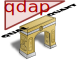
\includegraphics[width=3.5in]{imgs/qdaplogo.png}
\end{figure}

The \textbf{qdap} package \citep{R-qdap} is an R package designed to assist in quantitative discourse analysis. The package stands as a bridge between qualitative transcripts of dialogue and statistical analysis and visualization.  The \textbf{tm} package \citep{R-tm} is a major R \citep{R-core} package used for a variety of text mining tasks. Many text analysis packages have been built around the \textbf{tm} package's infrastructure (see \href{http://cran.r-project.org/web/views/NaturalLanguageProcessing.html}{CRAN Task View: Natural Language Processing}).  As \textbf{qdap} aims to act as a bridge to other R text mining analyses it is important that \textbf{qdap} provides a means of moving between the various \textbf{qdap} and \textbf{tm} data types.  

This vignette serves as a guide towards navigating between the \textbf{qdap} and \textbf{tm} packages.  Specifically, the two goals of this vignette are to (1) describe the various data formats of the two packages and (2) demonstrate the use of \textbf{qdap} functions that enable the user to move seamlessly between the two packages.




\newpage
\section{Data Formats}

\hspace{.4cm} The \textbf{qdap} and \textbf{tm} packages each have two basic data formats.  \textbf{qdap} stores raw text data in the form of a \texttt{data.frame} augmented with columns of demographic variables whereas \textbf{tm} stores raw text as a \texttt{Corpus} and annotates demographic information with Meta Data attributes.  The structures are both \texttt{list}s and are comparable.

The second format both packages use is a matrix structure of word frequency counts.  The \textbf{qdap} package utilizes the \emph{Word Frequency Matrix} (\texttt{wfm} function) whereas the \textbf{tm} package utilizes the \emph{Term Document Matrix} or \emph{Document Term Matrix} (\texttt{TermDocumentMatrix} and \texttt{DocumentTermMatrix} functions).  Again the structure is similar between these two data forms.  Table~\ref{datforms} lays out the data forms of the two packages.



\begin{singlespace}
\begin{table}[!ht]
\begin{center}
  \captionbox{\textbf{qdap}-\textbf{tm} Data forms \label{datforms}}{%
    \begin{tabular}{p{2cm}p{2cm}p{8cm}}
    \hline
    \multicolumn{1}{l}{Package} & \multicolumn{1}{l}{Raw Text} & \multicolumn{1}{l}{Word Counts}  \\
    \hline
    \noindent \textbf{qdap} & \noindent Dataframe & \noindent  Word Frequency Matrix \\
    \noindent \textbf{tm} & \noindent Corpus & \noindent Term Document Matrix/Document Term matrix \\
    \hline
    \end{tabular}
  }
\end{center}
\end{table}
\end{singlespace}

\noindent Figure~\ref{convert} provides a visual overview of the \textbf{qdap} functions used to convert between data structures.  Many of these conversion could be achieved via the \textbf{tm} package as well.

\begin{figure}[h!]
  \centering
    \includegraphics[width=4.60in]{imgs/data_convert.png}
    \caption{Converting Data between \textbf{qdap} and \textbf{tm}}
  \label{convert}
\end{figure}

One of the most visible differences between \textbf{qdap}-\textbf{tm} data forms is that \textbf{qdap} enables the user to readily view the data while the \textbf{tm} utilizes a print method that provides a summary of the data.  The \texttt{tm::inspect} function enables the user to view \textbf{tm} data forms. The \textbf{qdap} package provides \texttt{qdap::qview} and \texttt{qdap::htruncdf} functions to view more digestible amounts of the data. Let's have a look at the different data types.  We'll start by loading both packages:

\begin{knitrout}
\definecolor{shadecolor}{rgb}{0.969, 0.969, 0.969}\color{fgcolor}\begin{kframe}
\begin{alltt}
\hlkwd{library}\hlstd{(qdap);} \hlkwd{library}\hlstd{(tm)}
\end{alltt}
\end{kframe}
\end{knitrout}


\noindent Now let us have a look at the raw text storage of both packages. \\ 

\subsection{Raw Text}
\subsubsection{qdap's Raw Text}

\begin{knitrout}
\definecolor{shadecolor}{rgb}{0.969, 0.969, 0.969}\color{fgcolor}\begin{kframe}
\begin{alltt}
\hlstd{DATA}
\hlkwd{qview}\hlstd{(DATA)}
\hlkwd{htruncdf}\hlstd{(DATA)}
\end{alltt}
\end{kframe}
\end{knitrout}


\begin{knitrout}
\definecolor{shadecolor}{rgb}{0.969, 0.969, 0.969}\color{fgcolor}\begin{kframe}
\begin{alltt}
## > DATA
##
##        person sex adult                                 state code
## 1         sam   m     0         Computer is fun. Not too fun.   K1
## 2        greg   m     0               No it's not, it's dumb.   K2
## .
## .
## .
## 9       sally   f     0           What are you talking about?   K9
## 10 researcher   f     1         Shall we move on?  Good then.  K10
## 11       greg   m     0 I'm hungry.  Let's eat.  You already?  K11
\end{alltt}
\end{kframe}
\end{knitrout}

\begin{knitrout}
\definecolor{shadecolor}{rgb}{0.969, 0.969, 0.969}\color{fgcolor}\begin{kframe}
\begin{alltt}
## > qview(DATA)
##
## ========================================================================
## nrow =  11           ncol =  5             DATA
## ========================================================================
##        person sex adult      state code
## 1         sam   m     0 Computer i   K1
## 2        greg   m     0 No it's no   K2
## .
## .
## .
## 8         sam   m     0 I distrust   K8
## 9       sally   f     0 What are y   K9
## 10 researcher   f     1 Shall we m  K10
\end{alltt}
\end{kframe}
\end{knitrout}

\begin{knitrout}
\definecolor{shadecolor}{rgb}{0.969, 0.969, 0.969}\color{fgcolor}\begin{kframe}
\begin{alltt}
## > htruncdf(DATA)
##
##        person sex adult      state code
## 1         sam   m     0 Computer i   K1
## 2        greg   m     0 No it's no   K2
## .
## .
## .
## 8         sam   m     0 I distrust   K8
## 9       sally   f     0 What are y   K9
## 10 researcher   f     1 Shall we m  K10
\end{alltt}
\end{kframe}
\end{knitrout}

\subsubsection{tm's Raw Text}
\begin{knitrout}
\definecolor{shadecolor}{rgb}{0.969, 0.969, 0.969}\color{fgcolor}\begin{kframe}
\begin{alltt}
\hlkwd{data}\hlstd{(}\hlstr{"crude"}\hlstd{)}
\hlstd{crude}
\hlkwd{inspect}\hlstd{(crude)}
\end{alltt}
\end{kframe}
\end{knitrout}


\begin{knitrout}
\definecolor{shadecolor}{rgb}{0.969, 0.969, 0.969}\color{fgcolor}\begin{kframe}
\begin{alltt}
## > crude
## A corpus with 20 text documents
## 
## > crude[[1]]
## Diamond Shamrock Corp said that
## effective today it had cut its contract prices for crude oil by
## 1.50 dlrs a barrel.
##     The reduction brings its posted price for West Texas
## Intermediate to 16.00 dlrs a barrel, the copany said.
##     "The price reduction today was made in the light of falling
## .
## .
## .
##     Diamond is the latest in a line of U.S. oil companies that
## have cut its contract, or posted, prices over the last two days
## citing weak oil markets.
##  Reuter
\end{alltt}
\end{kframe}
\end{knitrout}

\subsection{Word/Term Frequency Counts}

\hspace{.4cm} Now we'll look at how the two packages handle word frequency counts.  We'll start by setting up the raw text forms the two packages expect.

\begin{knitrout}
\definecolor{shadecolor}{rgb}{0.969, 0.969, 0.969}\color{fgcolor}\begin{kframe}
\begin{alltt}
\hlstd{tm_dat} \hlkwb{<-} \hlstd{qdap_dat} \hlkwb{<-} \hlstd{DATA[}\hlnum{1}\hlopt{:}\hlnum{4}\hlstd{,} \hlkwd{c}\hlstd{(}\hlnum{1}\hlstd{,} \hlnum{4}\hlstd{)]}
\hlkwd{rownames}\hlstd{(tm_dat)} \hlkwb{<-} \hlkwd{paste}\hlstd{(}\hlstr{"docs"}\hlstd{,} \hlnum{1}\hlopt{:}\hlkwd{nrow}\hlstd{(tm_dat))}
\hlstd{tm_dat} \hlkwb{<-} \hlkwd{Corpus}\hlstd{(}\hlkwd{DataframeSource}\hlstd{(tm_dat[,} \hlnum{2}\hlstd{,} \hlkwc{drop}\hlstd{=}\hlnum{FALSE}\hlstd{]))}
\end{alltt}
\end{kframe}
\end{knitrout}

 
\noindent Both \texttt{qdap\_dat} and \texttt{tm\_dat} are storing this basic information:

\begin{knitrout}
\definecolor{shadecolor}{rgb}{0.969, 0.969, 0.969}\color{fgcolor}\begin{kframe}
\begin{verbatim}
##    person                         state
## 1     sam Computer is fun. Not too fun.
## 2    greg       No it's not, it's dumb.
## 3 teacher            What should we do?
## 4     sam          You liar, it stinks!
\end{verbatim}
\end{kframe}
\end{knitrout}


\newpage

\subsubsection{qdap's Frequency Counts}

\begin{knitrout}
\definecolor{shadecolor}{rgb}{0.969, 0.969, 0.969}\color{fgcolor}\begin{kframe}
\begin{alltt}
\hlkwd{with}\hlstd{(qdap_dat,} \hlkwd{wfm}\hlstd{(state, person))}
\end{alltt}
\end{kframe}
\end{knitrout}


\begin{knitrout}
\definecolor{shadecolor}{rgb}{0.969, 0.969, 0.969}\color{fgcolor}\begin{kframe}
\begin{verbatim}
##          greg researcher sally sam teacher
## computer    0          0     0   1       0
## do          0          0     0   0       1
## dumb        1          0     0   0       0
## fun         0          0     0   2       0
## is          0          0     0   1       0
## it          0          0     0   1       0
## it's        2          0     0   0       0
## liar        0          0     0   1       0
## no          1          0     0   0       0
## not         1          0     0   1       0
## should      0          0     0   0       1
## stinks      0          0     0   1       0
## too         0          0     0   1       0
## we          0          0     0   0       1
## what        0          0     0   0       1
## you         0          0     0   1       0
\end{verbatim}
\end{kframe}
\end{knitrout}



\subsubsection{tm's Frequency Counts}

\begin{knitrout}
\definecolor{shadecolor}{rgb}{0.969, 0.969, 0.969}\color{fgcolor}\begin{kframe}
\begin{alltt}
\hlkwd{TermDocumentMatrix}\hlstd{(tm_dat,}
    \hlkwc{control} \hlstd{=} \hlkwd{list}\hlstd{(}
        \hlkwc{removePunctuation} \hlstd{=} \hlnum{TRUE}\hlstd{,}
        \hlkwc{wordLengths}\hlstd{=}\hlkwd{c}\hlstd{(}\hlnum{0}\hlstd{,} \hlnum{Inf}\hlstd{)}
    \hlstd{)}
\hlstd{)}
\end{alltt}
\end{kframe}
\end{knitrout}


\begin{knitrout}
\definecolor{shadecolor}{rgb}{0.969, 0.969, 0.969}\color{fgcolor}\begin{kframe}
\begin{verbatim}
## A term-document matrix (16 terms, 4 documents)
## 
## Non-/sparse entries: 17/47
## Sparsity           : 73%
## Maximal term length: 8 
## Weighting          : term frequency (tf)
\end{verbatim}
\end{kframe}
\end{knitrout}


\noindent Now we'll Look at the tm output using \texttt{inspect}.

\begin{knitrout}
\definecolor{shadecolor}{rgb}{0.969, 0.969, 0.969}\color{fgcolor}\begin{kframe}
\begin{alltt}
\hlkwd{inspect}\hlstd{(}\hlkwd{TermDocumentMatrix}\hlstd{(tm_dat,}
    \hlkwc{control} \hlstd{=} \hlkwd{list}\hlstd{(}
        \hlkwc{removePunctuation} \hlstd{=} \hlnum{TRUE}\hlstd{,}
        \hlkwc{wordLengths}\hlstd{=}\hlkwd{c}\hlstd{(}\hlnum{0}\hlstd{,} \hlnum{Inf}\hlstd{)}
    \hlstd{)}
\hlstd{))}
\end{alltt}
\end{kframe}
\end{knitrout}


\begin{knitrout}
\definecolor{shadecolor}{rgb}{0.969, 0.969, 0.969}\color{fgcolor}\begin{kframe}
\begin{alltt}
##           Docs
## Terms      docs 1 docs 2 docs 3 docs 4
##   computer      1      0      0      0
##   do            0      0      1      0
##   dumb          0      1      0      0
##   fun           2      0      0      0
##   is            1      0      0      0
##   it            0      0      0      1
##   its           0      2      0      0
##   liar          0      0      0      1
##   no            0      1      0      0
##   not           1      1      0      0
##   should        0      0      1      0
##   stinks        0      0      0      1
##   too           1      0      0      0
##   we            0      0      1      0
##   what          0      0      1      0
##   you           0      0      0      1
\end{alltt}
\end{kframe}
\end{knitrout}

The two matrices are essentially the same, with the exception of column order and names.  Notice that by default \textbf{tm} removes words with fewer characters (word length) and does not discard punctuation (we made the matrices equal by specifying \texttt{removePunctuation = TRUE} and \texttt{wordLengths=c(0, Inf)} for \textbf{tm}'s \texttt{control} argument).  \textbf{qdap} takes the opposite approach, removing punctuation and utilizing all words, by default.  These differences arise out of the intended uses, audiences, and philosophies of the package authors.  Each has strengths in particular situations.  The \textbf{qdap} output is an ordinary \texttt{matrix} whereas the \textbf{tm} output is a more compact \texttt{simple triplet matrix}.  While the storage is different, both packages can be made to mimic the default of the other.  

Also note that the \textbf{qdap} \texttt{summary} method for \texttt{wfm} provides the user with information similar to the \texttt{TermDocumentMatrix}/\texttt{DocumentTermMatrix} functions' default \texttt{print} method.


\begin{knitrout}
\definecolor{shadecolor}{rgb}{0.969, 0.969, 0.969}\color{fgcolor}\begin{kframe}
\begin{alltt}
\hlkwd{summary}\hlstd{(}\hlkwd{with}\hlstd{(qdap_dat,} \hlkwd{wfm}\hlstd{(state, person)))}
\end{alltt}
\end{kframe}
\end{knitrout}


\begin{knitrout}
\definecolor{shadecolor}{rgb}{0.969, 0.969, 0.969}\color{fgcolor}\begin{kframe}


{\ttfamily\noindent\itshape\color{messagecolor}{\#\# A word-frequency matrix (16 terms, 5 groups)\\\#\# \\\#\# \\\#\# Non-/sparse entries\ \ \ \ \ \  : 17/63\\\#\# Sparsity\ \ \ \ \ \ \ \ \ \ \ \ \ \ \ \ \ \ : 79\%\\\#\# Maximal term length\ \ \ \ \ \  : 8\\\#\# Less than four characters : 56\%\\\#\# Hapax legomenon\ \ \ \ \ \ \ \ \ \  : 13(81\%)\\\#\# Dis legomenon\ \ \ \ \ \ \ \ \ \ \ \  : 3(19\%)\\\#\# Shannon's diversity index : 2.73}}\end{kframe}
\end{knitrout}


Now we'll look at some \textbf{qdap} functions that enable the user to move between packages, gaining the flexibility and benefits of both packages.


\section{Converting Data Forms}

\hspace{.4cm} We'll again use the following preset data.

\begin{knitrout}
\definecolor{shadecolor}{rgb}{0.969, 0.969, 0.969}\color{fgcolor}\begin{kframe}
\begin{alltt}
\hlstd{tm_dat} \hlkwb{<-} \hlstd{qdap_dat} \hlkwb{<-} \hlstd{DATA[}\hlnum{1}\hlopt{:}\hlnum{4}\hlstd{,} \hlkwd{c} \hlstd{(}\hlnum{1}\hlstd{,} \hlnum{4}\hlstd{) ]}
\hlkwd{rownames} \hlstd{(tm_dat)} \hlkwb{<-} \hlkwd{paste} \hlstd{(}\hlstr{"docs"}\hlstd{,} \hlnum{1}\hlopt{:} \hlkwd{nrow} \hlstd{(tm_dat))}
\hlstd{tm_dat} \hlkwb{<-} \hlkwd{Corpus} \hlstd{(} \hlkwd{DataframeSource} \hlstd{(tm_dat[,} \hlnum{2}\hlstd{,} \hlkwc{drop}\hlstd{=}\hlnum{FALSE}\hlstd{]))}

\hlstd{qdap_wfm} \hlkwb{<-} \hlkwd{with} \hlstd{(qdap_dat,} \hlkwd{wfm} \hlstd{(state, person))}
\hlstd{tm_tdm} \hlkwb{<-} \hlkwd{TermDocumentMatrix} \hlstd{(tm_dat,}
    \hlkwc{control} \hlstd{=} \hlkwd{list} \hlstd{(}
        \hlkwc{removePunctuation} \hlstd{=} \hlnum{TRUE}\hlstd{,}
        \hlkwc{wordLengths}\hlstd{=} \hlkwd{c} \hlstd{(}\hlnum{0}\hlstd{,} \hlnum{Inf}\hlstd{)}
    \hlstd{)}
\hlstd{)}
\end{alltt}
\end{kframe}
\end{knitrout}


\begin{enumerate}
  \item \texttt{qdap\_dat} -- is a \underline{\textbf{qdap} raw text} form
  \item \texttt{tm\_dat} -- is a \underline{\textbf{tm} raw text} format
  \item \texttt{qdap\_wfm} -- is a \underline{\textbf{qdap} word frequencies count}
  \item \texttt{tm\_tdm} -- is a \underline{\textbf{tm} word frequencies count}
\end{enumerate}

\noindent The reader is encouraged to view each of the data formats:

\begin{knitrout}
\definecolor{shadecolor}{rgb}{0.969, 0.969, 0.969}\color{fgcolor}\begin{kframe}
\begin{alltt}
\hlstd{qdap_dat;} \hlkwd{qview}\hlstd{(qdap_dat)}
\hlstd{tm_dat;} \hlkwd{inspect}\hlstd{(tm_dat)}
\hlstd{qdap_wfm;} \hlkwd{summary}\hlstd{(qdap_wfm)}
\hlstd{tm_tdm;} \hlkwd{inspect}\hlstd{(tm_tdm)}
\end{alltt}
\end{kframe}
\end{knitrout}


%%%%%%%%%%%%%%%%%%%%%%%%%%%

\subsection{Corpus to data.frame}

\hspace{.4cm} To move from a \texttt{Corpus} to a \texttt{data.frame} the \texttt{tm\_corpus2df} function is used as follows:

\begin{knitrout}
\definecolor{shadecolor}{rgb}{0.969, 0.969, 0.969}\color{fgcolor}\begin{kframe}
\begin{alltt}
\hlkwd{tm_corpus2df}\hlstd{(tm_dat)}
\end{alltt}
\end{kframe}
\end{knitrout}


\begin{knitrout}
\definecolor{shadecolor}{rgb}{0.969, 0.969, 0.969}\color{fgcolor}\begin{kframe}
\begin{verbatim}
##     docs tot                    text
## 1 docs 1 1.1        Computer is fun.
## 2 docs 1 1.2            Not too fun.
## 3 docs 2 2.1 No it's not, it's dumb.
## 4 docs 3 3.1      What should we do?
## 5 docs 4 4.1    You liar, it stinks!
\end{verbatim}
\end{kframe}
\end{knitrout}


\subsection{data.frame to Corpus}

\hspace{.4cm} To move from a \texttt{data.frame} to a \texttt{Corpus} the \texttt{df2tm\_corpus} function is used as follows:

\begin{knitrout}
\definecolor{shadecolor}{rgb}{0.969, 0.969, 0.969}\color{fgcolor}\begin{kframe}
\begin{alltt}
\hlkwd{with}\hlstd{(qdap_dat,} \hlkwd{df2tm_corpus}\hlstd{(state, person))}
\end{alltt}
\end{kframe}
\end{knitrout}


\begin{knitrout}
\definecolor{shadecolor}{rgb}{0.969, 0.969, 0.969}\color{fgcolor}\begin{kframe}
\begin{verbatim}
## A corpus with 3 text documents
\end{verbatim}
\end{kframe}
\end{knitrout}


\scriptsize\noindent *Note the 3 text documents; one for each grouping variable.  To get one for each row use: \\ \indent \texttt{with(qdap\_dat, df2tm\_corpus(state, id(person)))} \normalsize

\subsection{TermDocumentMatrix/DocumentTermMatrix to wfm}

\hspace{.4cm} To move from a \texttt{TermDocumentMatrix} to a \texttt{wfm} the \texttt{as.wfm} function is used as follows:

\begin{knitrout}
\definecolor{shadecolor}{rgb}{0.969, 0.969, 0.969}\color{fgcolor}\begin{kframe}
\begin{alltt}
\hlkwd{as.wfm}\hlstd{(tm_tdm)}
\end{alltt}
\end{kframe}
\end{knitrout}


\begin{knitrout}
\definecolor{shadecolor}{rgb}{0.969, 0.969, 0.969}\color{fgcolor}\begin{kframe}
\begin{verbatim}
##          docs 1 docs 2 docs 3 docs 4
## computer      1      0      0      0
## do            0      0      1      0
## dumb          0      1      0      0
## fun           2      0      0      0
## is            1      0      0      0
## it            0      0      0      1
## its           0      2      0      0
## liar          0      0      0      1
## no            0      1      0      0
## not           1      1      0      0
## should        0      0      1      0
## stinks        0      0      0      1
## too           1      0      0      0
## we            0      0      1      0
## what          0      0      1      0
## you           0      0      0      1
\end{verbatim}
\end{kframe}
\end{knitrout}



\subsection{wfm to TermDocumentMatrix/DocumentTermMatrix}

\hspace{.4cm} To move from a \texttt{wfm} to a \texttt{TermDocumentMatrix} or \texttt{DocumentTermMatrix} the \texttt{tdm} and \texttt{dtm} functions can be used as follows:

\begin{knitrout}
\definecolor{shadecolor}{rgb}{0.969, 0.969, 0.969}\color{fgcolor}\begin{kframe}
\begin{alltt}
\hlkwd{tdm}\hlstd{(qdap_wfm)}
\hlkwd{dtm}\hlstd{(qdap_wfm)}
\end{alltt}
\end{kframe}
\end{knitrout}


\begin{knitrout}
\definecolor{shadecolor}{rgb}{0.969, 0.969, 0.969}\color{fgcolor}\begin{kframe}
\begin{verbatim}
## A term-document matrix (16 terms, 5 documents)
## 
## Non-/sparse entries: 17/63
## Sparsity           : 79%
## Maximal term length: 8 
## Weighting          : term frequency (tf)
\end{verbatim}
\end{kframe}
\end{knitrout}


\begin{knitrout}
\definecolor{shadecolor}{rgb}{0.969, 0.969, 0.969}\color{fgcolor}\begin{kframe}
\begin{verbatim}
## A document-term matrix (5 documents, 16 terms)
## 
## Non-/sparse entries: 17/63
## Sparsity           : 79%
## Maximal term length: 8 
## Weighting          : term frequency (tf)
\end{verbatim}
\end{kframe}
\end{knitrout}


\subsection{Corpus to wfm}

\hspace{.4cm} One can also move directly from a \textbf{tm} \texttt{Corpus} to a \textbf{qdap} \texttt{wfm} with the \texttt{tm\_corpus2wfm} function.

\begin{knitrout}
\definecolor{shadecolor}{rgb}{0.969, 0.969, 0.969}\color{fgcolor}\begin{kframe}
\begin{alltt}
\hlkwd{tm_corpus2wfm}\hlstd{(tm_dat)}
\end{alltt}
\end{kframe}
\end{knitrout}


\begin{knitrout}
\definecolor{shadecolor}{rgb}{0.969, 0.969, 0.969}\color{fgcolor}\begin{kframe}
\begin{verbatim}
##          docs 1 docs 2 docs 3 docs 4
## computer      1      0      0      0
## do            0      0      1      0
## dumb          0      1      0      0
## fun           2      0      0      0
## is            1      0      0      0
## it            0      0      0      1
## it's          0      2      0      0
## liar          0      0      0      1
## no            0      1      0      0
## not           1      1      0      0
## should        0      0      1      0
## stinks        0      0      0      1
## too           1      0      0      0
## we            0      0      1      0
## what          0      0      1      0
## you           0      0      0      1
\end{verbatim}
\end{kframe}
\end{knitrout}


\section{Stemming, Stopwords, and Choosing n-Character Words/Terms from a wfm}


\hspace{.4cm} Many of the \textbf{qdap} and \textbf{tm} functions have means of stemming, removing stopwords, and bounding, that is filtering rows (greater than, equal to or less than) meeting min/max criteria.  \textbf{qdap} also offers two external functions to address these issues directly.  


\subsection{stemming}

\hspace{.4cm} \textbf{qdap} takes the approach that the user stems the dataframe upon creation (using \texttt{sentSplit(..., stem = TRUE)}) or after (using the \texttt{stem2df} function), maintaining a column of stemmed and unstemmed text for various analyses.

\begin{knitrout}
\definecolor{shadecolor}{rgb}{0.969, 0.969, 0.969}\color{fgcolor}\begin{kframe}
\begin{alltt}
\hlkwd{sentSplit}\hlstd{(qdap_dat,} \hlstr{"state"}\hlstd{,} \hlkwc{stem} \hlstd{=} \hlnum{TRUE}\hlstd{)}
\end{alltt}
\end{kframe}
\end{knitrout}


\begin{knitrout}
\definecolor{shadecolor}{rgb}{0.969, 0.969, 0.969}\color{fgcolor}\begin{kframe}
\begin{verbatim}
##    person tot                   state          stem.text
## 1     sam 1.1        Computer is fun.     Comput is fun.
## 2     sam 1.2            Not too fun.       Not too fun.
## 3    greg 2.1 No it's not, it's dumb. No it not it dumb.
## 4 teacher 3.1      What should we do? What should we do?
## 5     sam 4.1    You liar, it stinks! You liar it stink!
\end{verbatim}
\end{kframe}
\end{knitrout}



\subsection{Filtering: Stopwords and Bounding}
    

\hspace{.4cm} \textbf{qdap}'s \texttt{Filter} function allows the user to remove stopwords and bound a Word Frequency Matrix (\texttt {wfm}).  First we'll construct a minimal Word Frequency Matrix:

\begin{knitrout}
\definecolor{shadecolor}{rgb}{0.969, 0.969, 0.969}\color{fgcolor}\begin{kframe}
\begin{alltt}
\hlstd{qdap_wfm} \hlkwb{<-} \hlkwd{with}\hlstd{(qdap_dat,} \hlkwd{wfm}\hlstd{(state, person))}
\end{alltt}
\end{kframe}
\end{knitrout}


\begin{knitrout}
\definecolor{shadecolor}{rgb}{0.969, 0.969, 0.969}\color{fgcolor}\begin{kframe}
\begin{verbatim}
##          greg researcher sally sam teacher
## computer    0          0     0   1       0
## do          0          0     0   0       1
## dumb        1          0     0   0       0
## fun         0          0     0   2       0
## is          0          0     0   1       0
## it          0          0     0   1       0
## it's        2          0     0   0       0
## liar        0          0     0   1       0
## no          1          0     0   0       0
## not         1          0     0   1       0
## should      0          0     0   0       1
## stinks      0          0     0   1       0
## too         0          0     0   1       0
## we          0          0     0   0       1
## what        0          0     0   0       1
## you         0          0     0   1       0
\end{verbatim}
\end{kframe}
\end{knitrout}


Now we'll move through a series of examples demonstrating the usage of \texttt{Filter} on a \texttt{wfm} object.


\begin{knitrout}
\definecolor{shadecolor}{rgb}{0.969, 0.969, 0.969}\color{fgcolor}\begin{kframe}
\begin{alltt}
\hlkwd{Filter}\hlstd{(qdap_wfm,} \hlkwc{min} \hlstd{=} \hlnum{5}\hlstd{)}
\end{alltt}
\end{kframe}
\end{knitrout}



\begin{knitrout}
\definecolor{shadecolor}{rgb}{0.969, 0.969, 0.969}\color{fgcolor}\begin{kframe}
\begin{verbatim}
##          greg researcher sally sam teacher
## computer    0          0     0   1       0
## should      0          0     0   0       1
## stinks      0          0     0   1       0
\end{verbatim}
\end{kframe}
\end{knitrout}



\begin{knitrout}
\definecolor{shadecolor}{rgb}{0.969, 0.969, 0.969}\color{fgcolor}\begin{kframe}
\begin{alltt}
\hlkwd{Filter}\hlstd{(qdap_wfm,} \hlkwc{min} \hlstd{=} \hlnum{5}\hlstd{,} \hlkwc{max} \hlstd{=} \hlnum{7}\hlstd{)}
\end{alltt}
\end{kframe}
\end{knitrout}


\begin{knitrout}
\definecolor{shadecolor}{rgb}{0.969, 0.969, 0.969}\color{fgcolor}\begin{kframe}
\begin{verbatim}
##        greg researcher sally sam teacher
## should    0          0     0   0       1
## stinks    0          0     0   1       0
\end{verbatim}
\end{kframe}
\end{knitrout}


\begin{knitrout}
\definecolor{shadecolor}{rgb}{0.969, 0.969, 0.969}\color{fgcolor}\begin{kframe}
\begin{alltt}
\hlkwd{Filter}\hlstd{(qdap_wfm,} \hlnum{4}\hlstd{,} \hlnum{4}\hlstd{)}
\end{alltt}
\end{kframe}
\end{knitrout}


\begin{knitrout}
\definecolor{shadecolor}{rgb}{0.969, 0.969, 0.969}\color{fgcolor}\begin{kframe}
\begin{verbatim}
##      greg researcher sally sam teacher
## dumb    1          0     0   0       0
## it's    2          0     0   0       0
## liar    0          0     0   1       0
## what    0          0     0   0       1
\end{verbatim}
\end{kframe}
\end{knitrout}


\begin{knitrout}
\definecolor{shadecolor}{rgb}{0.969, 0.969, 0.969}\color{fgcolor}\begin{kframe}
\begin{alltt}
\hlkwd{Filter}\hlstd{(qdap_wfm,} \hlnum{4}\hlstd{,} \hlnum{4}\hlstd{,} \hlkwc{count.apostrophe} \hlstd{=} \hlnum{FALSE}\hlstd{)}
\end{alltt}
\end{kframe}
\end{knitrout}


\begin{knitrout}
\definecolor{shadecolor}{rgb}{0.969, 0.969, 0.969}\color{fgcolor}\begin{kframe}
\begin{verbatim}
##      greg researcher sally sam teacher
## dumb    1          0     0   0       0
## liar    0          0     0   1       0
## what    0          0     0   0       1
\end{verbatim}
\end{kframe}
\end{knitrout}


\begin{knitrout}
\definecolor{shadecolor}{rgb}{0.969, 0.969, 0.969}\color{fgcolor}\begin{kframe}
\begin{alltt}
\hlkwd{Filter}\hlstd{(qdap_wfm,} \hlnum{3}\hlstd{,} \hlnum{4}\hlstd{)}
\end{alltt}
\end{kframe}
\end{knitrout}


\begin{knitrout}
\definecolor{shadecolor}{rgb}{0.969, 0.969, 0.969}\color{fgcolor}\begin{kframe}
\begin{verbatim}
##      greg researcher sally sam teacher
## dumb    1          0     0   0       0
## fun     0          0     0   2       0
## it's    2          0     0   0       0
## liar    0          0     0   1       0
## not     1          0     0   1       0
## too     0          0     0   1       0
## what    0          0     0   0       1
## you     0          0     0   1       0
\end{verbatim}
\end{kframe}
\end{knitrout}


\begin{knitrout}
\definecolor{shadecolor}{rgb}{0.969, 0.969, 0.969}\color{fgcolor}\begin{kframe}
\begin{alltt}
\hlkwd{Filter}\hlstd{(qdap_wfm,} \hlnum{3}\hlstd{,} \hlnum{4}\hlstd{,} \hlkwc{stopwords} \hlstd{= Top200Words)}
\end{alltt}
\end{kframe}
\end{knitrout}


\begin{knitrout}
\definecolor{shadecolor}{rgb}{0.969, 0.969, 0.969}\color{fgcolor}\begin{kframe}
\begin{verbatim}
##      greg researcher sally sam teacher
## dumb    1          0     0   0       0
## fun     0          0     0   2       0
## it's    2          0     0   0       0
## liar    0          0     0   1       0
\end{verbatim}
\end{kframe}
\end{knitrout}



\section{Apply Functions Intended for TermDocumentMatrix to wfm Object}

\hspace{.4cm} At times it is convenient to apply a function intended for a \textbf{tm} \texttt{TermDocumentMatrix} or \texttt{DocumentTermMatrix} directly to a \textbf{qdap} \texttt{wfm} object.  \textbf{qdap}'s \texttt{apply\_as\_tm} function enables these functions to be used directly on a \texttt{wfm}.

\subsection{A Minimal wfm Object}

\hspace{.4cm} Let us begin with a slightly larger \texttt{wfm} minimal example:

\begin{knitrout}
\definecolor{shadecolor}{rgb}{0.969, 0.969, 0.969}\color{fgcolor}\begin{kframe}
\begin{alltt}
\hlstd{a} \hlkwb{<-} \hlkwd{with}\hlstd{(DATA,} \hlkwd{wfm}\hlstd{(state,} \hlkwd{list}\hlstd{(sex, adult)))}
\end{alltt}
\end{kframe}
\end{knitrout}


\begin{knitrout}
\definecolor{shadecolor}{rgb}{0.969, 0.969, 0.969}\color{fgcolor}\begin{kframe}


{\ttfamily\noindent\itshape\color{messagecolor}{\#\# A word-frequency matrix (41 terms, 4 groups)\\\#\# \\\#\# \\\#\# Non-/sparse entries\ \ \ \ \ \  : 45/119\\\#\# Sparsity\ \ \ \ \ \ \ \ \ \ \ \ \ \ \ \ \ \ : 73\%\\\#\# Maximal term length\ \ \ \ \ \  : 8\\\#\# Less than four characters : 49\%\\\#\# Hapax legomenon\ \ \ \ \ \ \ \ \ \  : 32(78\%)\\\#\# Dis legomenon\ \ \ \ \ \ \ \ \ \ \ \  : 7(17\%)\\\#\# Shannon's diversity index : 3.62}}\end{kframe}
\end{knitrout}



\subsection{A Small Demonstration}

\hspace{.4cm} Here we will use the \textbf{tm} package's \texttt{removeSparseTerms} to remove sparse terms from a \texttt{wfm} object and return a Word Frequency Matrix object (\texttt{wfm} class).

\begin{knitrout}
\definecolor{shadecolor}{rgb}{0.969, 0.969, 0.969}\color{fgcolor}\begin{kframe}
\begin{alltt}
\hlstd{out} \hlkwb{<-} \hlkwd{apply_as_tm}\hlstd{(a, tm::removeSparseTerms,} \hlkwc{sparse}\hlstd{=}\hlnum{0.6}\hlstd{)}
\end{alltt}
\end{kframe}
\end{knitrout}


\begin{knitrout}
\definecolor{shadecolor}{rgb}{0.969, 0.969, 0.969}\color{fgcolor}\begin{kframe}
\begin{alltt}
\hlkwd{summary}\hlstd{(out)}
\end{alltt}
\end{kframe}
\end{knitrout}


\begin{knitrout}
\definecolor{shadecolor}{rgb}{0.969, 0.969, 0.969}\color{fgcolor}\begin{kframe}


{\ttfamily\noindent\itshape\color{messagecolor}{\#\# A word-frequency matrix (3 terms, 4 groups)\\\#\# \\\#\# \\\#\# Non-/sparse entries\ \ \ \ \ \  : 7/5\\\#\# Sparsity\ \ \ \ \ \ \ \ \ \ \ \ \ \ \ \ \ \ : 42\%\\\#\# Maximal term length\ \ \ \ \ \  : 4\\\#\# Less than four characters : 67\%\\\#\# Hapax legomenon\ \ \ \ \ \ \ \ \ \  : 0(0\%)\\\#\# Dis legomenon\ \ \ \ \ \ \ \ \ \ \ \  : 1(33\%)\\\#\# Shannon's diversity index : 1.06}}\end{kframe}
\end{knitrout}


\begin{knitrout}
\definecolor{shadecolor}{rgb}{0.969, 0.969, 0.969}\color{fgcolor}\begin{kframe}
\begin{alltt}
\hlkwd{class}\hlstd{(out)}
\end{alltt}
\end{kframe}
\end{knitrout}


\begin{knitrout}
\definecolor{shadecolor}{rgb}{0.969, 0.969, 0.969}\color{fgcolor}\begin{kframe}
\begin{verbatim}
## [1] "wfm"         "true.matrix" "matrix"
\end{verbatim}
\end{kframe}
\end{knitrout}


\subsection{Further Examples to Try}

Here are some further examples to try:

\begin{knitrout}
\definecolor{shadecolor}{rgb}{0.969, 0.969, 0.969}\color{fgcolor}\begin{kframe}
\begin{alltt}
\hlkwd{apply_as_tm}\hlstd{(a, tm::dissimilarity,} \hlkwc{method} \hlstd{=} \hlstr{"cosine"}\hlstd{)}
\hlkwd{apply_as_tm}\hlstd{(a, tm::findAssocs,} \hlstr{"computer"}\hlstd{,} \hlnum{.8}\hlstd{)}
\hlkwd{apply_as_tm}\hlstd{(a, tm::findFreqTerms,} \hlnum{2}\hlstd{,} \hlnum{3}\hlstd{)}
\hlkwd{apply_as_tm}\hlstd{(a, tm::Zipf_plot)}
\hlkwd{apply_as_tm}\hlstd{(a, tm::Heaps_plot)}
\hlkwd{apply_as_tm}\hlstd{(a, tm::plot.TermDocumentMatrix,} \hlkwc{corThreshold} \hlstd{=} \hlnum{0.4}\hlstd{)}

\hlkwd{library}\hlstd{(proxy)}
\hlkwd{apply_as_tm}\hlstd{(a, tm::weightBin)}
\hlkwd{apply_as_tm}\hlstd{(a, tm::weightBin,} \hlkwc{to.qdap} \hlstd{=} \hlnum{FALSE}\hlstd{)}
\hlkwd{apply_as_tm}\hlstd{(a, tm::weightSMART)}
\hlkwd{apply_as_tm}\hlstd{(a, tm::weightTfIdf)}
\end{alltt}
\end{kframe}
\end{knitrout}


\section{Apply Functions Intended for qdap Dataframes to tm Corpus}

\hspace{.4cm} While the \textbf{tm} package (and other packages used on \textbf{tm} objects) tends to conduct analysis by feeding functions a \texttt{TermDocumentMatrix} or \texttt{DocumentTermMatrix} \textbf{qdap} generally feeds functions raw text directly.  There are advantages to both approaches (e.g., the matrix is a mathematical structure while raw text maintains word order).  Many \textbf{qdap} functions can be used on the \texttt{Corpus} structure via the \texttt{apply\_as\_df} function.    

\subsection{A Small Demonstration}

\hspace{.4cm} Here we will use the \textbf{qdap} package's \texttt{trans\_cloud} function, on our minimal \textbf{tm} \texttt{Corpus}, to produce a word cloud with particular words highlighted:

\begin{knitrout}
\definecolor{shadecolor}{rgb}{0.969, 0.969, 0.969}\color{fgcolor}\begin{kframe}
\begin{alltt}
\hlstd{matches} \hlkwb{<-} \hlkwd{list}\hlstd{(}
    \hlkwc{good} \hlstd{=} \hlstr{"fun"}\hlstd{,}
    \hlkwc{bad} \hlstd{=} \hlkwd{c}\hlstd{(}\hlstr{"dumb"}\hlstd{,} \hlstr{"stinks"}\hlstd{,} \hlstr{"liar"}\hlstd{)}
\hlstd{)}

\hlkwd{apply_as_df}\hlstd{(tm_dat, trans_cloud,} \hlkwc{grouping.var}\hlstd{=}\hlkwa{NULL}\hlstd{,}
    \hlkwc{target.words}\hlstd{=matches,} \hlkwc{cloud.colors} \hlstd{=} \hlkwd{c}\hlstd{(}\hlstr{"red"}\hlstd{,} \hlstr{"blue"}\hlstd{,} \hlstr{"grey75"}\hlstd{))}
\end{alltt}
\end{kframe}
\end{knitrout}


\begin{knitrout}
\definecolor{shadecolor}{rgb}{0.969, 0.969, 0.969}\color{fgcolor}

{\centering \includegraphics[width=\maxwidth]{figure/minimal-apply_as_df2} 

}



\end{knitrout}


\subsection{Further Examples to Try}

\hspace{.4cm} Here are some further examples to try:

\begin{knitrout}
\definecolor{shadecolor}{rgb}{0.969, 0.969, 0.969}\color{fgcolor}\begin{kframe}
\begin{alltt}
\hlkwd{library}\hlstd{(tm)}
\hlstd{reut21578} \hlkwb{<-} \hlkwd{system.file}\hlstd{(}\hlstr{"texts"}\hlstd{,} \hlstr{"crude"}\hlstd{,} \hlkwc{package} \hlstd{=} \hlstr{"tm"}\hlstd{)}
\hlstd{reuters} \hlkwb{<-} \hlkwd{Corpus}\hlstd{(}\hlkwd{DirSource}\hlstd{(reut21578),}
    \hlkwc{readerControl} \hlstd{=} \hlkwd{list}\hlstd{(}\hlkwc{reader} \hlstd{= readReut21578XML))}

\hlkwd{apply_as_df}\hlstd{(reuters, word_stats)}
\hlkwd{apply_as_df}\hlstd{(reuters, formality)}
\hlkwd{apply_as_df}\hlstd{(reuters, word_list)}
\hlkwd{apply_as_df}\hlstd{(reuters, polarity)}
\hlkwd{apply_as_df}\hlstd{(reuters, Dissimilarity)}
\hlkwd{apply_as_df}\hlstd{(reuters, diversity)}
\hlkwd{apply_as_df}\hlstd{(tm_dat, pos_by)}
\hlkwd{apply_as_df}\hlstd{(reuters, flesch_kincaid)}
\hlkwd{apply_as_df}\hlstd{(tm_dat, trans_venn)}
\hlkwd{apply_as_df}\hlstd{(reuters, gantt_plot)}
\hlkwd{apply_as_df}\hlstd{(reuters, rank_freq_mplot)}
\hlkwd{apply_as_df}\hlstd{(reuters, character_table)}
\hlkwd{apply_as_df}\hlstd{(reuters, trans_cloud)}

\hlstd{matches2} \hlkwb{<-} \hlkwd{list}\hlstd{(}
    \hlkwc{oil} \hlstd{=} \hlkwd{qcv}\hlstd{(oil, crude),}
    \hlkwc{money} \hlstd{=} \hlkwd{c}\hlstd{(}\hlstr{"economic"}\hlstd{,} \hlstr{"money"}\hlstd{)}
\hlstd{)}

\hlstd{(termco_out} \hlkwb{<-} \hlkwd{apply_as_df}\hlstd{(reuters, termco,} \hlkwc{match.list} \hlstd{= matches2))}
\hlkwd{plot}\hlstd{(termco_out,} \hlkwc{values} \hlstd{=} \hlnum{TRUE}\hlstd{,} \hlkwc{high}\hlstd{=}\hlstr{"red"}\hlstd{)}

\hlstd{(wordcor_out} \hlkwb{<-} \hlkwd{apply_as_df}\hlstd{(reuters, word_cor,} \hlkwc{word} \hlstd{=} \hlkwd{unlist}\hlstd{(matches2)))}
\hlkwd{plot}\hlstd{(wordcor_out)}

\hlstd{(f_terms} \hlkwb{<-} \hlkwd{apply_as_df}\hlstd{(reuters, freq_terms,} \hlkwc{at.least} \hlstd{=} \hlnum{3}\hlstd{))}
\hlkwd{plot}\hlstd{(f_terms)}

\hlstd{finds} \hlkwb{<-} \hlkwd{apply_as_df}\hlstd{(reuters, freq_terms,} \hlkwc{at.least} \hlstd{=} \hlnum{5}\hlstd{,}
    \hlkwc{top} \hlstd{=} \hlnum{5}\hlstd{,} \hlkwc{stopwords} \hlstd{= Top100Words)}
\hlkwd{apply_as_df}\hlstd{(reuters, dispersion_plot,} \hlkwc{match.terms} \hlstd{= finds[,} \hlnum{1}\hlstd{],}
    \hlkwc{total.color} \hlstd{=} \hlkwa{NULL}\hlstd{)}
\end{alltt}
\end{kframe}
\end{knitrout}


\section{Conclusion}

\hspace{.4cm} This vignette described the various data formats for the \textbf{qdap} and \textbf{tm} packages.  It also demonstrated some of the basic functionality of the \textbf{qdap} functions designed to navigate between the two packages.  For more information on the \textbf{tm} package \citep{Feinerer2008} use:

\begin{knitrout}
\definecolor{shadecolor}{rgb}{0.969, 0.969, 0.969}\color{fgcolor}\begin{kframe}
\begin{alltt}
\hlkwd{browseVignettes}\hlstd{(}\hlkwc{package} \hlstd{=} \hlstr{"tm"}\hlstd{)}
\end{alltt}
\end{kframe}
\end{knitrout}


\noindent Likewise, the user may view additional information about the \textbf{qdap} package \citep{R-qdap}:

\begin{knitrout}
\definecolor{shadecolor}{rgb}{0.969, 0.969, 0.969}\color{fgcolor}\begin{kframe}
\begin{alltt}
\hlkwd{browseVignettes}\hlstd{(}\hlkwc{package} \hlstd{=} \hlstr{"qdap"}\hlstd{)}
\end{alltt}
\end{kframe}
\end{knitrout}



\section*{Acknowledgments}

\textbf{qdap} relies heavily on the \textbf{tm} package.  The \textbf{tm} package has extended text analysis to the R platform.  Thank you to Ingo Feinerer and Kurt Hornik for their work on this and many other R packages. \\

\noindent This document was produced with \textbf{knitr} \citep{R-knitr}.  Thank you to Yihui Xie for the \textbf{knitr} package and as well as his many other contributions to the R community.


\bibliographystyle{jss}
\bibliography{qdap}

\end{document}













